%!TEX root = ./../thesis.tex

\chapter{State Centric Programming Model}
\label{c:state_centric}
Most state-of-the-art frameworks for distributed machine learning like Petuum \cite{Xing2015} and Parameter Server \cite{Li2014} are based on the parameter server concept introduced in the previous section.
The framework essentially provides a low level API\footnote{Application programming interface} for publishing and retrieving values similar to a distributed key-value store, where the key $i$ is for example the index of a weight vector $w$ stored on the server and the value is the weight $w_i$.
Implementing an algorithm that relies on a parameter server requires to incorporate the publishing and retrieval of parameters deeply into the algorithm.
This contrasts the general workflow of developing and testing an algorithm locally on a single machine and then transition to a distributed environment.
The parameter server paradigm provides only a minor abstraction, leaving the developer with the task of distributing state, scheduling distributed computation, consistency management and managing cluster resources.
A developer should be able to focus on the key elements to efficient parallel execution of distributed machine learning algorithms.
In the following section these key elements of a framework that improves upon currently available systems are derived by the help of an example based on elastic-net regularized linear regression.
The result is a state centric programming model, treating state as a first class citizen that can be distributed and altered by local and remote transformation.

\section{Control Flow}

Figure \ref{fig:general_pipeline} shows the logical control flow of a general pipeline for training an arbitrary iterative-convergent machine learning algorithm.
\begin{figure}[ht]
\centering
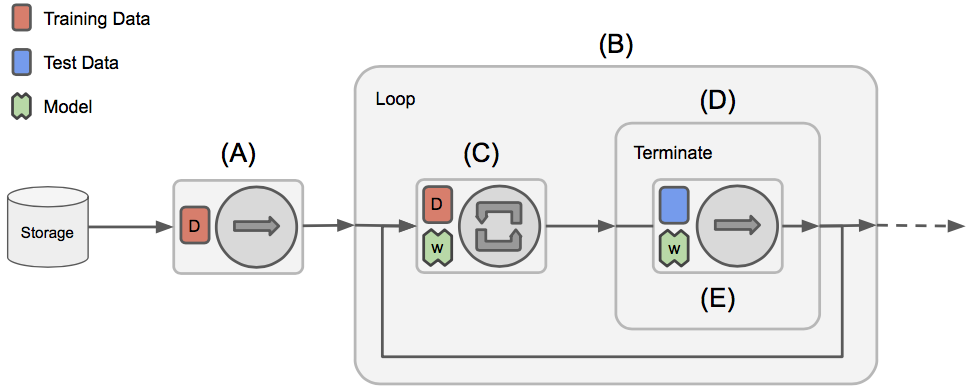
\includegraphics[width=0.9\textwidth]{img/general_pipeline.png}
\caption{Machine Learning Pipeline for iterative-convergent algorithms}
\label{fig:general_pipeline}
\end{figure}
Usually training starts with loading the input data $D$ from the storage followed by one ore more preprocessing steps (e.g. normalization or standardization) as well as splitting the data into training and test set \textbf{(A)}.
A square represents a step of an algorithm, which contains an arbitrary number of input states (e.g. data, model) and some kind of transformation applied to the input states.
The transformation process is depicted as a circle and can either be applied once (arrow) or multiple times (cyclic arrows) to the input state(s) during this particular step.
After applying the preprocessing the actual training process is triggered, which is commonly contained in a loop \textbf{(B)}.
A loop symbolises that the containing steps are executed repeatedly until some termination criterion is statisfied, which is computed in \textbf{(C)}.
For most machine learning algorithms the termination criterion can either be a fixed number of iterations, the change in objective $Q$ between iterations or the generalization performance \textbf{(E)}.
\textbf{(D)} is the actual training step which iteratively refines the model by updates computed from the input data according to \ref{eqn:delta_upd}.
It can already be seen from the example that a framework for distributed machine learning must be capable of consicely expressing a complex sequence of arbitrary control flow operators and transformation steps.
An algorithm expressed in this form can be executed as is on a single machine without modification but in order to distribute it among a cluster of machines each transformation step must be parallelized as can be seen in Figure \ref{fig:general_pipeline_dist}.
\textbf{NOTE:} add caption for state, make termination more generic, it's better to call this control flow
\begin{figure}[ht]
\centering
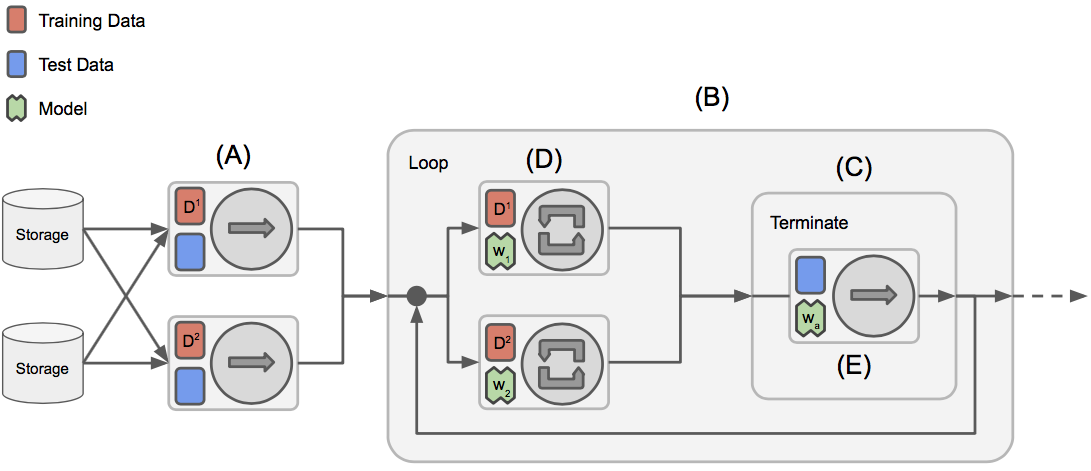
\includegraphics[width=0.9\textwidth]{img/general_pipeline_dist.png}
\caption{Distributed Machine Learning Pipeline for Iterative-convergent Algorithms}
\label{fig:general_pipeline_dist}
\end{figure}
The pipeline described in Figure \ref{fig:general_pipeline} is parallelized with a degree of parallelism of two.
Now each transformation step of the pipeline can be scheduled and executed on two machines in parallel.
It is worth noting that the transformation logic stays the same independently of the dop\footnote{degree of parallelism}, including a dop of one, which is essentially a single machine.
Only the input and output state(s) of each step have changed in a sense that each parallel step only has access to a part of the orginal state.

\section{Distributed State}
Therefore the actual concern in distributed machine learning is not how to distribute computation but how to distribute the state in order to achieve optimal performance.
As this thesis focuses on machine learning, a state is in general represented by a tensor (e.g. vector or matrix).
The most efficient state distribution depends on properties of the state(s) such as size and sparsity of the input data and model, algorithm used for optimization and infrastructure properties such as available memory and computational resources.


\section{Consistency}

NOTES:
- motivate the argumentation with an example machine learning pipeline (elastic-net linear regression) which includes preprocessing (e.g. standard-scaling), iterative model refinement which could be data/model parallel and depending on the size of the model it could either be replicated or partitioned among machines/workers, also a ML pipeline involves generalization error assessment via test/validation dataset, which should be included into the stopping criterion
this should show:
	- what kind of workflow is generaly executed in practice
	- what structure a ml pipeline has and that there are parts that can be run in parallel and in parallel with relaxed constistency/synchronization
	- show what kind of information can be infered from knowledge about the architecture (computational and memory resources, bandwidth, bandwidth quota) and the problem size (size of input data, size of model)
	- what part of distributing a machine learning algorithm can be handled by the system (distributing data, distributing model and computation, scheduling of work) and what needs to be specified by the developer (parallelism, control flow and required states (?), )

- describe the limitations of current state-of-the-art distributed machine learning systems
	- low level primitives
	- not flexible nor expressible api for developing real word machine learning pipelines
	- inference of certain properties depending on hardware architecture (GPU, CPU, FPGA) and algorithm properties
	- distributed control flow
	- focus on optimizing distributed machine learning performance by quick prototyping
	- only concerned with the important parts for going from an exact single machine to a distributed algorithm implementation by specifying data partitioning, topology and constistency management properties (synchronzation requirements/schemes, filter, update/merging strategies)
	- dealing with algorithm related hyperparameters
